% Need to review Justin Grimmer

\chapter{Computational Social Science}
\label{ch:css}

While the previous chapters were mostly retrospective analyses, computational
social science is mostly in the ``here and now''.  It is focus on data
being generated in the past hours, days, or weeks to inform
inteligence analysists, brand monitors, journalists, or social
scientists.  The underlying problem is the same, however: these
stakeholders are interested in what people have to say but cannot read
all of the data at their disposal.

Historically, social science questions such as what candidates is
prefered in a particular part of the country or whether people like a
new restaurant or product were answered by polling: social scientists
would head out into the world, gather a statistically significant
sample, and extrapolate to the broader population.

These techniques are still valuable, but they still take time.  A
company needs to know if it has an issue with a product immediately,
particularly if its good name is being dragged through the mud on
social media~\cite{bowen-16}.  However, the reason for the acute time
pressure can also be the solution: if a company is able to quickly see
that it has a social media problem, it can more quickly intervene and
correct the issue.

Traditional social science methods are labor intensive, take a long
time, or are impossible for sensitive subjects.  For instance, surveys
of influenza take too long to be useful compared to the life cycle of
influenza's progression~\cite{broniatowsky-15}; using twitter and
Google searches results in more accurate information faster.

Monitoring pollution in China or drug use in teens requires access to
populations that may be difficult.  Using social media presents an
alternative~\cite{wang:paul:dredze-15}, as individuals share
information more freely than official news agencies (which may suffer
from censorship) or in school-administered surveys (which can suffer
from self-sensorship).  Topic models and other large-data approaches
that can look at vast quantities of text help overcome some of the
obstacles to fast-response social science.

\section{Sentiment Analysis}

In industrial settings, this problem is often called sentiment
analysis~\citep{pang-08}.  Here, the goal is to determine the
``sentiment''---e.g., positive or negative opinions---associated with
a piece of text.  For example, ``Chipotle is great!'' would be
associated with positive sentiment, while ``Chipotle made me sick
would be associated with negative sentiment''.

While indistrial applications of sentiment analysis is mostly for
identifying whether people like a product or copany, there are wider
social science applications of examining large corpora to determine
authors' \emph{internal state}.  For example, determining whether they
they are politically liberal or conservative based on their online
commentary.

Topic models can help these tasks by dividing a problem into topics.
For example, ``Apple'' can appear in tech news as well as a food
ingredient; someone monitoring the seller of iPods and iPhones would
not want to be confused by social media commentary complaining about a
bad apple pie.  ``surprising'' in an automotive review is likely
associated with negative seintment, while it's a good thing in a book
review.  Thus, topics can help differentiate different kinds of
discussion in broad corpora.

However, topic models lose their value if you want to \emph{contrast}
sentiment within a topic.  While a topic model can find people
discussing Chipotle burritos online, it cannot separate the lovers from
haters.  Thus, \emph{distinguishing} topics based on their sentiment
can help a user better understand how topics and sentiment interact in
a dataset.  This requires modifying the topic model to make it aware
of the underlying sentiment.

% Sentiment is an example of meta data, which can be visualized to
% better understand a corpus (see viz).

\section{Upstream and Downstream Models}

To distinguish topics based on their sentiment, the model must be
aware of what sentiment is.  In the language of probabilistic models,
sentiment and topic are modeled \emph{jointly}.  That is, there is a
probability distribution over both the sentiment of a document $y$ and
the topics that is uses $z$.

There are two general kinds of joint models that incorporate metadata
such as sentiment: upstream and downstream models.  The distinction is
based on the generative story of topic models (Chapter~\ref{ch:intro}): is
sentiment before (upstream) or after (downstream) topics in the
generative story?

% Put in graphical model examples of upstream and downstream models

Upstream models assume that sentiment comes first in the generative
story.  That is, there will be different topics given the underlying
sentiment.  This can come in the form in a prior learned from observed
sentiment~\citep{mimno-08} or from a latent variable that can serve as
a proxy for sentiment~\citep{lin-09}.  Upstream models are often
easier to implement and are more flexible~\citep{stewart-14}.

In contrast, downstream models explicitly predict sentiment
\emph{given} text.  If the goal is the later predict sentiment given
raw text with the help of topic models, downstream models can work
better than upstream models.  These models are often called
``supervised'' topic models after supervised
\abr{lda}~\citep{blei-07b}, which use a document's topics to predict
the downstream sentiment regression: a document's sentiment~$y_d$ is
assumed to come from a normal distribution with mean $\eta^\top \bar
z$, where $\bar z$ is a normalized vector of all of the topics that a
document uses and $\eta$ is a regression parameter that describes the
sentiment of each topic.

During inference, the words and sentiments work together to find
combinations of topic and sentiment that make sense.  While
``vanilla'' topic models seek to find clusters of words that make
sense together, if a topic is associated with documents with many
different sentiment values, it will have low probability.  

\begin{figure}
  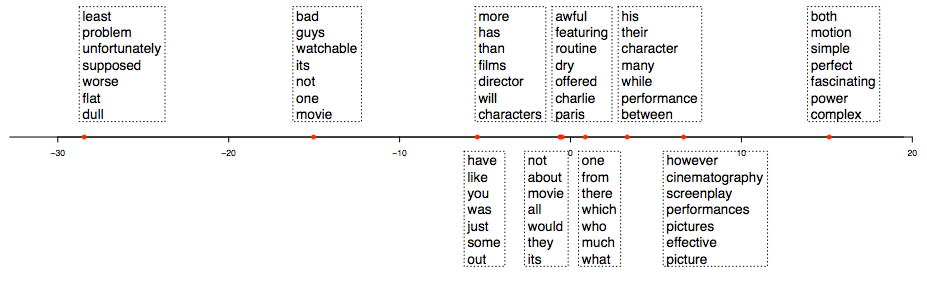
\includegraphics[width=0.7\linewidth]{figures/slda}
  \caption{Example topics learned by supervised \abr{lda} from
    \citet{blei-07b}.  Each topic is not just a collection of words
    but also has a regression score~$\eta$ that explains whether it is
    associated with positive sentiment (right) or negative sentiment
    (left).}
\end{figure}

Consider Figure~\ref{fig:slda-topics}.  If a topic has an inconsistent
sentiment values (for example, a negative sentiment document in a
positive sentiment topic), inference will try to move the negative
sentiment documents to topics with consistent sentiment~$\eta$ {\bf
  and} consistent words.  

These models form the foundation for the models and problems we
discuss in the rest of this section.

\paragraph{Aside: Prediction or Interpretation}

A common theme in using topic models is the emphasis on whether models
should prioritize \emph{prediction} or \emph{interpretation}.  Our
previous chapters have focused on interpretation: can a user
understand the output of a model?  But for supervised models, there's
a question of how well the model can predict $y_d$ (sentiment or
another prediction of interest).  

To some extent, these are not always in conflict.  \citet{ramage-10b}
show that topic model features can improve tweet categorization, as
do \citet{blei-07b} for supervised \abr{lda}.  However, changing the
objective function can further improve predictions~\citep{zhu-09}.

However, sometimes improved interpretability hampers the ability of
the model to predict content.  This is true of both words within a
document and document labels.  \citet{chang-09b} showed that
complicated topic models do a better job of predicting held-out
documents but make less sense to a user.  \citet{Nguyen-15:anchor}
show that supervised models offer better predictions with additional
topics but the topics are less interpretable.

\section{Understanding Stance and Polarization}

Another form of internal state is \emph{stance}: which side does a
person take on an issue.  This can take many forms: are you for or
against a proposal, are you a Democrat or a Republican, or are you a
fan of the original Star Trek or the new version?

Upstream models can discover these sides by incorporating stance into
the generative model.  For example, \citet{paul-10} posit that each
``side'' had a distribution over words that it uses generally
\emph{and} that each side had its own take on how it discusses a
topic.  Within a document, each word is chosen either from a side's
background distribution, a side's version of the topic, or from the
topic's ``neutral'' words.  For instance, Israelis and Palestinians
both use ``attacks'', ``civilians'', and ``military'' in discussing
unrest in Israeli-occupied Palestine, but the Israeli side uses
``terrorist'' and ``incitement'', while the Palestinean side focuses
on ``resistance'' and ``occupation''.

Downstream models can also capture these divisions as well.
\citet{nguyen-13:shlda} predict whether a speaker is Republican or
Democrat based on the versions of topics they discuss.  For example,
Republicans are more likely to discuss taxes in general than
Democrats, but Democrats focus on the good that comes out of taxes
(Figure~\cite{fig:shlda-taxes}).

However, there are not always two sides to an issue.  A probabilistic
solution to this model is the nested Dirichlet
process~\citep{blei-07}.  These hierarchies induce a non parametric
hierarchy over an unbounded number of topics.  This corresponds to
agenda setting from political
science~\citep{Nguyen:Boyd-Graber:Resnik:Miler-2015}.

% Eisenstein

\section{Social Networks}

We have talked about meta data that are independent for each user.
Sometimes, however, we are interested in meta data that describe the
relationships between people

This makes modeling more difficult, but we still see the same division
between upstream and downstream models

The stochastic block model is the prototype for upstream models~\cite{airoldi-08}

Link LDA is the exemplar for downstream models~\cite{nallapati-08}

Hybrid models can have the best of both worlds

Supervised LDA bases regressions on the topic assignments rather than
the allocations.  Doing something similar can also improve link prediction~\citep{chang-09a}

But changing the objective function can improve performance further~\cite{bach-15}

This can discover geographic variation in language~\cite{eisenstein-10}



But what if we are interested in regions with multiple languages or
dialects?
